\documentclass{agujournal}
\journalname{Journal of Advances in Modeling Earth Systems (JAMES)}
\usepackage{graphicx}
\usepackage{subcaption}
\usepackage{amsmath}
\usepackage{hyperref}
\usepackage[table]{xcolor}
\hypersetup{colorlinks=true,citecolor=black,filecolor=black,linkcolor=black,urlcolor=black,breaklinks=true}
\usepackage{natbib}
\bibpunct{(}{)}{;}{a}{,}{,~}
\hyphenation{ILAMB}
\hyphenation{CARDAMOM}

\newcommand{\bx}{\mathbf{x}}
\DeclareMathOperator*{\argmax}{arg\,max}

\begin{document}

\title{The International Land Model Benchmarking (ILAMB) System: Observational Uncertainty}

\authors{Nathan~Collier\affil{1},
	Morgan~Steckler\affil{1},
	Forrest~M.~Hoffman\affil{1,2},
	David~M.~Lawrence\affil{3}}

\affiliation{1}{Computational Science and Engineering Division, Oak Ridge National Laboratory, Oak Ridge, TN, USA}
\affiliation{2}{Department of Civil \& Environmental Engineering, University of Tennessee, Knoxville, TN, USA}
\affiliation{3}{Climate \& Global Dynamics Division, National Center for Atmospheric Research, Boulder, CO, USA}

\correspondingauthor{Nathan Collier}{nathaniel.collier@gmail.com}

\begin{abstract}
	Blah
\end{abstract}

\section{Introduction}\label{sec:intro}

This is a paper about including reference data uncertainty when synthesizing model performance. In~\cite{Collier_JAMES_20181101} we detailed a methodology developed by and employed in the International Land Model Benchmarking (ILAMB) effort. While the ideas presented here will be presented in the context of our previous work, we believe the principles presented will be of value to the broader benchmarking community.

Modelers and analysts use benchmarking tools and software (cite[ESMValTool,PMP,others]) to evaulate model predictions with respect to reference data. To evaluate performance these packages calculate metrics such as bias and RMSE among others representing mismatch between models and reference data. While we frequently attribute the cause of a high bias or RMSE to a departure of the model data from the reference, it can also be because of reference data uncertainty. This is an important detail to consider as models errors lead model developers to focus on parameterization improvements. If we report large errors in areas where the reference data is uncertain, then we mislead this develpoment.

To address this problem we propose a change to the ILAMB methodology that accounts for reference uncertainty when given. In section~\ref{t:datasets} we will describe a collection of global or continental scale datasets that provide explicit measures of uncertainty. However, we note that the while more datasets express uncertainty, the source or object of that uncertainty varies. In some cases, these reference datasets are built by merging multiple sources and the uncertainty relates to the variance among these products. In others, samples collected in sparse and discrete locations are extended to the globe by mapping to representative regions and the uncertainty is represented as the spread among measurements per region.

Due to this ambiguity, we do not want to make structural assumptions about what the uncertainty constitutes. For this reason our methodology will adopt a simple ``perfect in the envelope'' paradigm. This means that if a model variable time series falls within the reference data uncertainty range, then the models performance is indistruishable from a ``perfect'' model. While a useful phrasing shorthand, it is not that we declare models flawless if in the envlope of uncertainty. It is rather that we do not wish to lead model developers to resolve an error about which we are not certain is really an error.

In this paper, we propse a modification to the ILAMB scoring methodology for the bias and RMSE aspects to include notions of the reference uncertainty when present. We approach this change with four philosophical goals in mind:
%
\begin{enumerate}
	\item As the uncertainty tends to zero, the proposed additions should reduce to the original ILAMB methodoloy for each aspect. While there are an increasing number of reference datasets with some measure of uncertainty, the majority do not. Layering in uncertainty in this way lets us understand and interpret results with and without uncertainty within the same framework.
	\item As the meaning or intrepretation of uncertainty varies in each data product, we should use a simple approach and make no assumptions about its structure.
	\item The methodological changes should only affect how we synthesize errors (score) and not affect raw error or other scalars we report.
	\item For a given model location (or pixel), the proposed methodology should never degrade the score. The uncertainty should make us more conservative about judgements. This in turn also means that a perfect score no longer represents a flawless match to the reference data, but rather indicates a limit to the conclusions we can draw from a given reference dataset.
\end{enumerate}

\section{Methodology}\label{sec:method}

The ILAMB scoring methodology aims to synthesize model performance with respect to a reference in several aspects including bias, root mean squared error (RMSE), annual cycle, and spatial distribution. The goal is to be comprehensive and provide a uniform high level summary of the performance of these models. To this end, we have developed expressions~\cite{Collier_JAMES_20181101} that synthesize the model performance in each aspect, reducing errors to a single \textit{score} that varies from 0 to 1, indicating poor and perfect performance respectively.

As in~\cite{Collier_JAMES_20181101}, we discuss the analysis of a generalized variable $v(t,\bx)$ which we assume represents a piecewise discontinuous function of constants in space and time. This means that the temporal domain, represented by the variable $t$, is defined by the beginning $t_0$ and ending $t_f$ of time intervals and the spatial domain, represented by the variable $\bx$ (bolded to emphasize it is a vector quantity), represents the areas created by cell boundaries or the areas associated with data sites. A single overbar denotes a temporal mean, expressed as an integral,
%
\begin{equation}
	\bar{v}(\bx) = \frac{1}{t_f-t_0} \int_{t_0}^{t_f} v(t,\bx)\ dt\label{e:mean}
\end{equation}
%
The exposition below will also make use of centralized versions of variables which we will denote by a hat symbol,
%
\begin{equation}
	\widehat{v}(t,\bx) = v(t,\bx)-\bar{v}(\bx)\label{e:center}
\end{equation}
%
When necessary, we use the subscript `ref' to reflect a variable whose source is a reference or observational dataset, and the subscript `com' for the comparison or model datasets. We approach changes to our methodology assuming that we have a comparison (model) variable $v_{\mathrm{com}}(t,\bx)$ and reference variable $v_{\mathrm{ref}}(t,\bx)$ with uncertainty given at each space-time location $\delta(t,\bx)$. For simplicity in this exposition, we will assume that the uncertainty represents a kind of standard error. However, uneven interval style uncertainty such as those represented by confidence intervals can be used with simple additions to the implementation.

In general, the ILAMB methodology develops a spatial measure of relative error $\varepsilon(\bx)$ and then converts this to a score through the exponential,
%
\begin{equation}
	s(\bx) = e^{-\varepsilon(\bx)}\label{e:score}
\end{equation}
%
This part of the procedure will remain unchanged. In the following subsections we modify the expressions of relative error for each aspect.

\subsection{Bias}

In~\cite{Collier_JAMES_20181101} the relative error for the bias is given as,
%
\begin{equation}
	\varepsilon^{p}_{\mathrm{bias}}(\bx) = \frac{\left| \overline{v_{\mathrm{com}}}(\bx) -\overline{v_{\mathrm{ref}}}(\bx) \right|}{\mathrm{std}_t\left( v_{\mathrm{ref}}(t,\bx)\right)}\label{e:bias0}
\end{equation}
%
In words, we compute the relative error by dividing the absolute value of the bias by the standard deviation in time of the reference data. That is, the size of the bias is normalized by how much variation is present at each spatial location. To avoid confusion with expressions derived in this paper, we use a superscript $p$ to indicate that this was the previous expression. We propose the following change to the bias relative error:

\begin{equation}
	\varepsilon_{\mathrm{bias}}(\bx) = \frac{\max\left(\left| \overline{v_{\mathrm{com}}}(\bx) -\overline{v_{\mathrm{ref}}}(\bx) \right|-\overline{\delta}(\bx),0\right)}{\mathrm{std}_t\left( v_{\mathrm{ref}}(t,\bx)\right)}\label{e:bias}
\end{equation}

This means that we substract the mean reference uncertainty from the bias and only count where this expression is greater than 0. In the limit that the uncertainty is zero, $\overline{\delta}(\bx)=0$, the numerator reduces to the absolute value of the bias recovering to equation~\eqref{e:bias0}. In this interpretation, the uncertainty functions as an error discount also leading to scores that will not degrade.

\begin{figure}[htbp]
	\centering
	\begin{subfigure}[t]{0.495\textwidth}
		\centering
		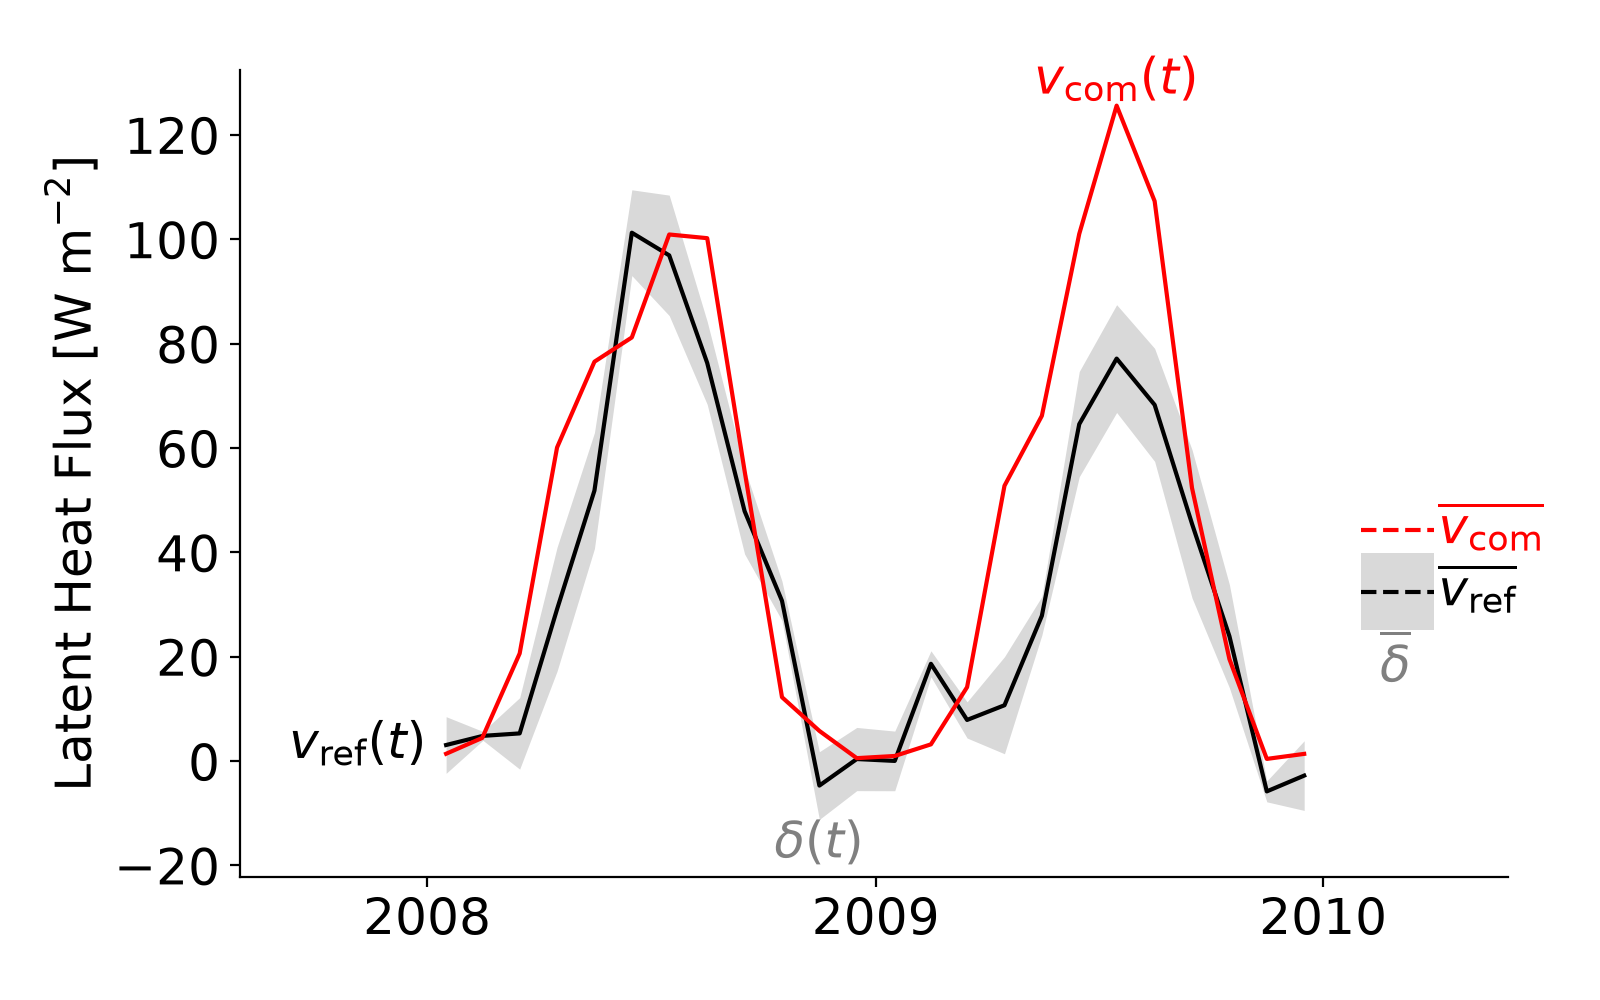
\includegraphics[width=\textwidth]{../figs/bias_moderate.png}
		\caption{Relatively low uncertainty leads to moderate gains in bias score (0.696 to 0.872) as shown in equation~\eqref{e:biasA}. Only the bias that falls outside the uncertainty envelope is penalized.}
		\label{fig:modbias}
	\end{subfigure}
	\hfill
	\begin{subfigure}[t]{0.495\textwidth}
		\centering
		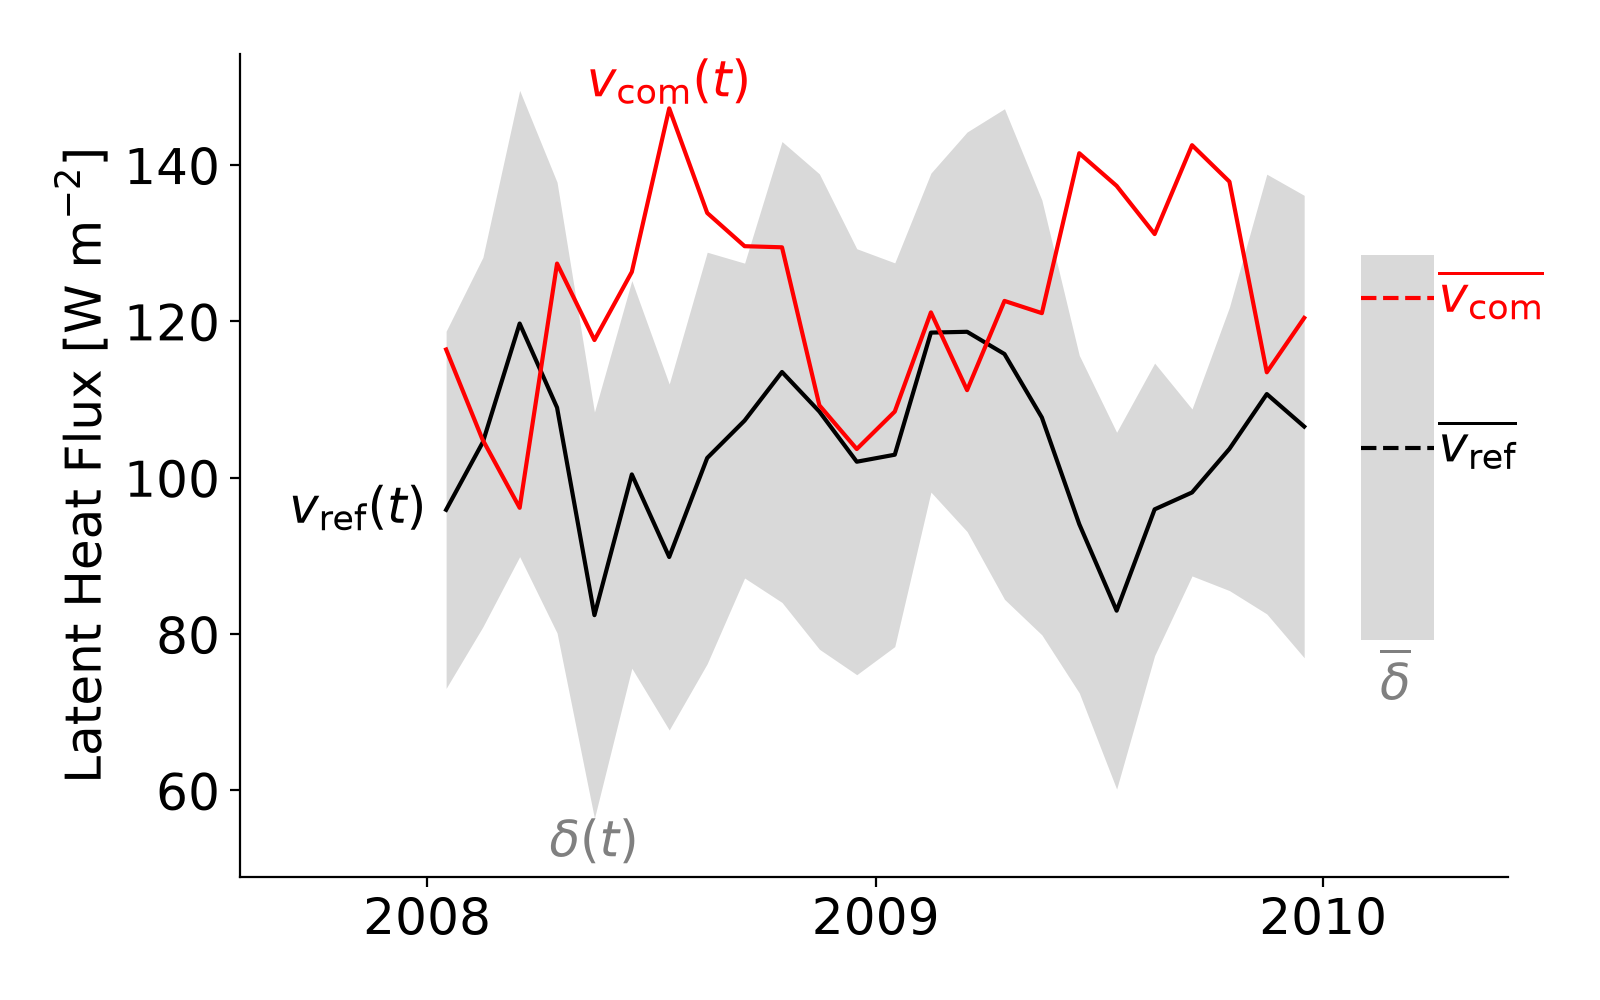
\includegraphics[width=\textwidth]{../figs/bias_large.png}
		\caption{Even a large bias which falls within the uncertainty envelope leads to a perfect bias score (0.147 to 1.0) as shown in equation~\eqref{e:biasB}.}
		\label{fig:bigbias}
	\end{subfigure}
	\caption{Sample illustrations of how uncertainty affects the ILAMB scoring methodology for the bias at particular grid cells. In each case the reference variable $v_{\mathrm{ref}}(t)$ is shown in black along with its uncertainty $\delta(t)$ shaded grey. The comparison variable $v_{\mathrm{com}}(t)$ is shown in red. The temporal mean of each is shown to the right of the plot and indicated by a bar over the corresponding variable.}
	\label{fig:bias}
\end{figure}
%
To develop some intuition in how these formulas work and compare to the previous definitions, consider the following case study comparing the latent heat provided by the CLASS (\cite{Hobeichi_JClim_20200301}) dataset to that of CanESM5 compared at two locations. One location, site A, is in central Canada and corresponds to a place where the uncertainty is relatively low. The other location, site B, is in Indonesia and corresponds to a place with poor model characterization and high uncertainty. Two years of the time trace at both sites is shown in figure~\ref{fig:bias}.

The time series for Site A are shown in figure~\ref{fig:modbias}. As we have selected values at a site, the dependence on $\bx$ has been dropped. While the model captures the major trends of the reference datasaet, there is a positive bias shown by the dashed lines to the right of the plot. However, there is also some reference uncertainty to consider also. If we harvest values from these datasets and substitute into equations~\eqref{e:bias0},~\eqref{e:bias}, and \eqref{e:score}, we get the following scores.
%
\begin{subequations}
	\label{e:biasA}
	\begin{align}
		\overline{v_{\mathrm{ref}}}                 & = 32.4                                                           \\
		\overline{v_{\mathrm{com}}}                 & = 44.3                                                           \\
		\mathrm{std}_t\left(v_{\mathrm{ref}}\right) & = 32.8                                                           \\
		\overline{\delta}                           & = 7.378                                                          \\
		\varepsilon^{p}                             & = \frac{\left| 44.3 - 32.4 \right|}{32.8}                = 0.363 \\
		\varepsilon                                 & = \frac{\max(\left| 44.3 - 32.4 \right| - 7.4,0)}{32.8}  = 0.137 \\
		s^{p}_{\mathrm{bias}}                       & = e^{-0.363} = 0.696                                             \\
		s_{\mathrm{bias}}                           & = e^{-0.137} = 0.872
	\end{align}
\end{subequations}
%
So by also considering the reference uncertainty, our score in this location has changed from 0.696 to 0.872. In constrast, consider the traces for site B shown in figure~\ref{fig:bigbias}. We can extract data from these time traces and make the same comparison as with site A.
%
\begin{subequations}
	\label{e:biasB}
	\begin{align}
		\overline{v_{\mathrm{ref}}}                 & = 103.8                                                       \\
		\overline{v_{\mathrm{com}}}                 & = 123.0                                                       \\
		\mathrm{std}_t\left(v_{\mathrm{ref}}\right) & = 10.0                                                        \\
		\overline{\delta}                           & = 24.6                                                        \\
		\varepsilon^{p}                             & = \frac{\left| 123- 103.8 \right|}{10.0}               = 1.92 \\
		\varepsilon                                 & = \frac{\max(\left| 123-103.8\right| - 24.6,0)}{10.0}  = 0    \\
		s^{p}_{\mathrm{bias}}                       & = e^{-1.92} = 0.147                                           \\
		s_{\mathrm{bias}}                           & = e^{0} = 1
	\end{align}
\end{subequations}
%
The model in this case does a poor job at capturing the mean behavior of the reference data leading to a significant positive bias and a low score of 0.147. However, once we consider how uncertain the reference data is in this location, this score is improved to 1.0. This does not mean that the model is perfect or that there is no more work to be done in improving parameterizations. It rather means that we have reached the interpretative limit of what this dataset can tell us in this location.
%
\subsection{RMSE}
%
We address uncertainty in scoring the RMSE in a similar fashion. In~\cite{Collier_JAMES_20181101} the relative error for the RMSE is given as,
%
\begin{equation}
	\varepsilon^{p}_{\mathrm{rmse}}(\bx) =
	\sqrt{\int_{t_0}^{t_f}
		\left(\widehat{v_{\mathrm{com}}}(t,\bx)-\widehat{v_{\mathrm{ref}}}(t,\bx)\right)^2
		\ dt} \bigg/
	\sqrt{\int_{t_0}^{t_f}
		\left(\widehat{v_{\mathrm{ref}}}(t,\bx)\right)^2
		\ dt}
	\label{e:rmse0}
\end{equation}
%
where the $1/(t_f-t_0)$ terms have been dropped as they cancel out. Note that when developing the RMSE score, we use the centralized versions of the variables. This is because we wish to develop a score which necessarily correlates with bias. A large bias will always lead to a large RMSE and thus a model would be double penalized as we synthesize. By using the centralized variables, we subtract out the bias and remove one strong correlate.

We use the same idea as in the bias score, where we aim to only penalize errors that go beyond the uncertainty. In the case of RMSE we do this inside the integrand, leading to the follow change in relative error,
%
\begin{multline}
	\varepsilon_{\mathrm{rmse}}(\bx) =
	\sqrt{\int_{t_0}^{t_f}
		\left(\max\left(\left|\widehat{v_{\mathrm{com}}}(t,\bx)-\widehat{v_{\mathrm{ref}}}(t,\bx)\right|-\delta(t,\bx),0\right)\right)^2
		\ dt} \bigg/\\
	\sqrt{\int_{t_0}^{t_f}
		\left(\widehat{v_{\mathrm{ref}}}(t,\bx)\right)^2
		\ dt}
	\label{e:rmse}
\end{multline}
%
\begin{figure}[htbp]
	\centering
	\begin{subfigure}[t]{0.495\textwidth}
		\centering
		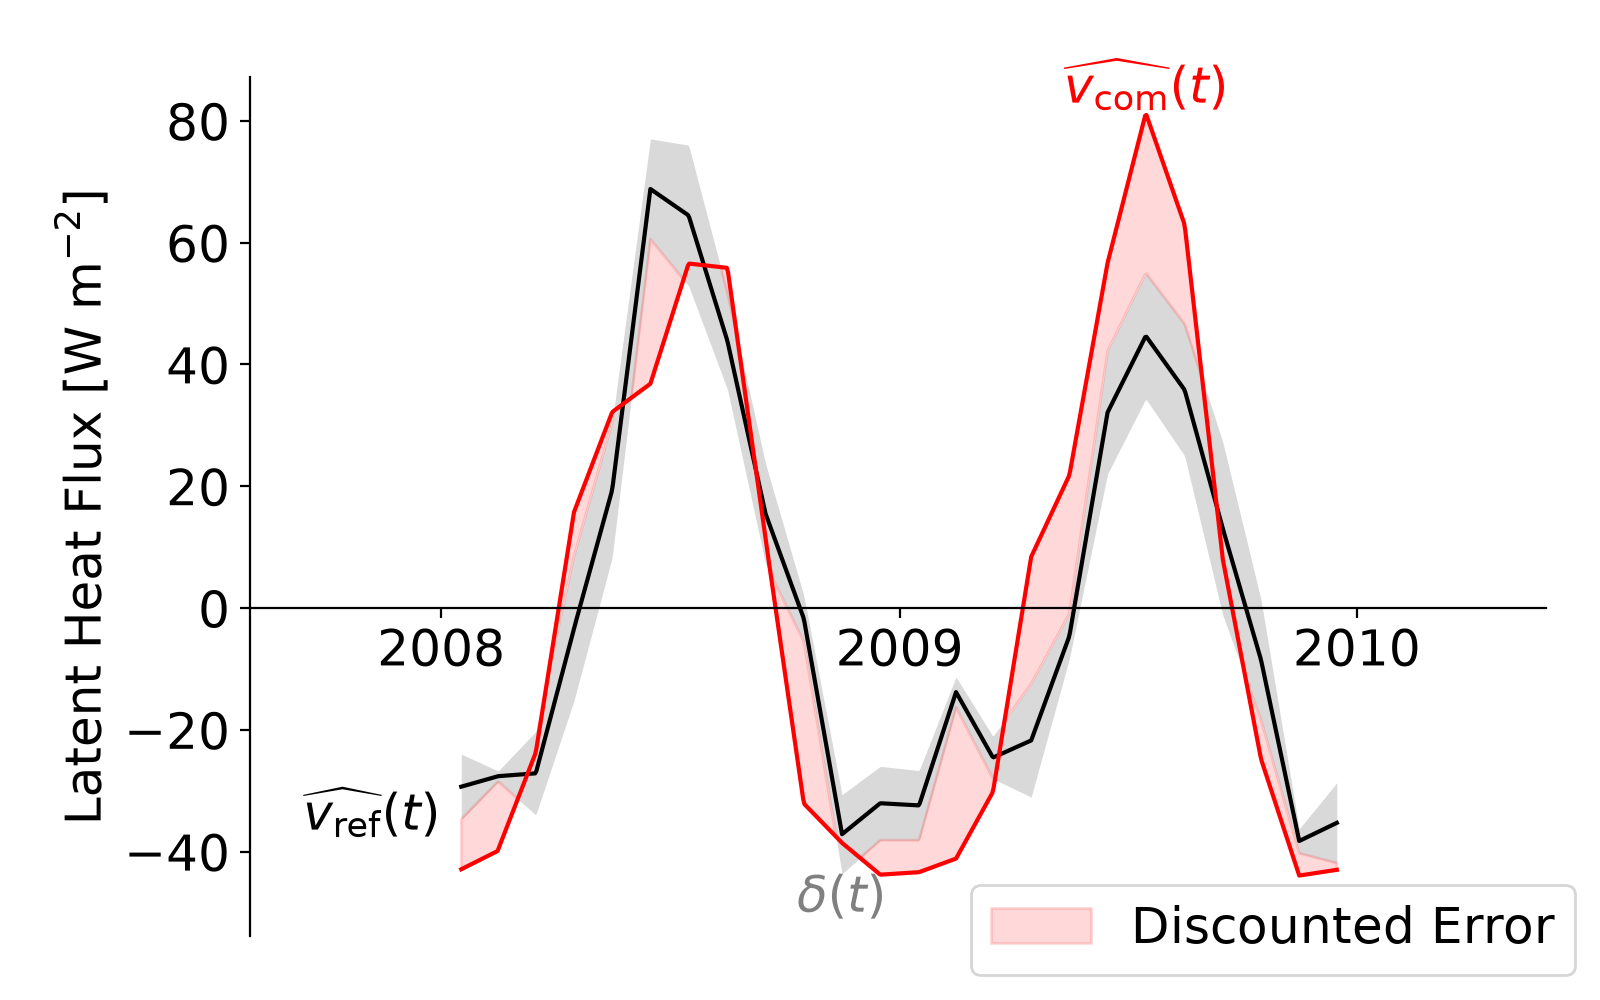
\includegraphics[width=\textwidth]{../figs/rmse_moderate.png}
		\caption{Moderate gains in RMSE score when the uncertainty is relatively low. The error that is squared and integrated is discounted by the reference uncertainty. Site chosen from central Canada.}
		\label{fig:modrmse}
	\end{subfigure}
	\hfill % Adds horizontal space between the two images
	% Second Subfigure
	\begin{subfigure}[t]{0.495\textwidth}
		\centering
		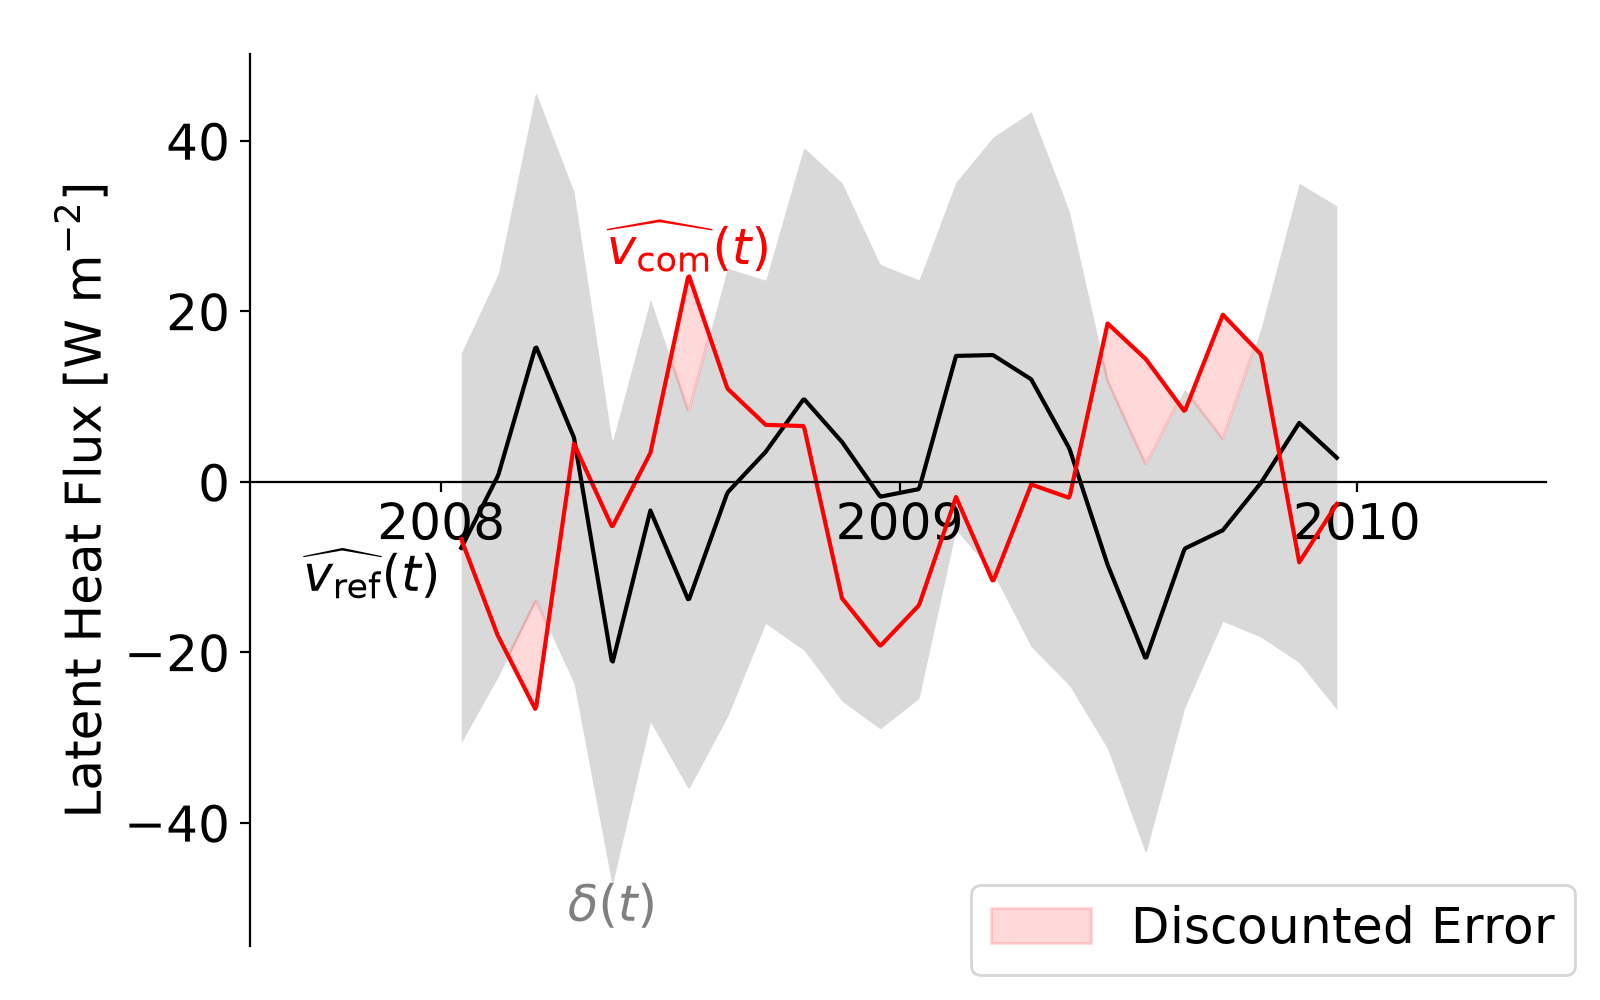
\includegraphics[width=\textwidth]{../figs/rmse_large.png}
		\caption{Large gains in RMSE score as the latent heat is highly uncertain. As the bias falls withing the uncertainty envelope, this site receives a perfect score. Site chosen from Indonesia.}
		\label{fig:bigrmse}
	\end{subfigure}
	\caption{Sample illustrations of how uncertainty affects the ILAMB scoring methodology for the RMSE at particular grid cells. In each case the reference variable $v_{\mathrm{ref}}(t)$ is shown in black along with its uncertainty $\delta(t)$ shaded grey. The comparison variable $v_{\mathrm{com}}(t)$ is shown in red. The temporal mean of each is shown to the right of the plot and indicated by a bar over the corresponding variable.}
	\label{fig:rmse}
\end{figure}
%
The interpretation of equation~\eqref{e:rmse} is straightforward to intuit in figure~\ref{fig:rmse} where we repeat the comparisons at the same two sites except the traces have been centralized. When computing $\varepsilon^p_{\mathrm{rmse}}(\bx)$ from equation~\eqref{e:rmse0}, the integral in the numerator is summing up the area between the red and black curve. In constrast, when computing $\varepsilon_{\mathrm{rmse}}(\bx)$ from equation~\eqref{e:rmse} only the light red shaded areas are included in the numerator's integral, leading to a discount in the total integrated error.

\clearpage
\section{Datasets}\label{sec:data}

While there are relatively few reference datasets that provide some explicit measure of uncertainty, the number is growing. In this section we will discuss these datasets starting with those produced by the same methodology and ending with unique products, highlighting the source of uncertainty in each case. We summarize the datasets included in this paper along with the variables available in each in table~\ref{t:datasets}.
\newcommand{\classvars}{
	precipitation ($\mathit{pr}$),
	evapotranspiration/latent heat ($\mathit{evspsbl}$/$\mathit{hfls}$),
	runoff ($\mathit{mrro}$),
	sensible heat ($\mathit{hfss}$),
	surface net radiation ($\mathit{rns}$)
}
\newcommand{\cardvars}{
	soil carbon ($\mathit{cSoil}$),
	evapotranspiration ($\mathit{evspsbl}$),
	carbon from fire ($\mathit{fFire}$),
	gross primary productivity ($\mathit{gpp}$),
	leaf area index ($\mathit{lai}$),
	surface runoff ($\mathit{mrros}$),
	runoff ($\mathit{mrro}$),
	net biome production ($\mathit{nbp}$),
	net ecosystem exchange ($\mathit{nee}$),
	autotrophic respiration ($\mathit{ra}$),
	heterotrophic respiration ($\mathit{rh}$),
	surface snow ($\mathit{snw}$),
	transpiration ($\mathit{tran}$)
}
\newcommand{\woavars}{
	oxygen ($\mathit{o2}$),
	nitrate ($\mathit{no3}$),
	phosphate ($\mathit{po4}$),
	silicate ($\mathit{si}$),
	temperature ($\mathit{thetao}$)
}
\begin{table}[ht]
	\caption{A selection of global or continental scale reference datasets which include some measure of uncertainty.}\label{t:datasets}
	\rowcolors{1}{white}{gray!15}
	\begin{tabular}{llp{7cm}}
		\hline
		Section            & Dataset           & Variables                                                                            \\
		\hline
		\ref{s:cardamom}   & CARDAMOM          & \cardvars                                                                            \\
		\ref{s:olc}        & CLASS-1-1         & \classvars                                                                           \\
		\ref{s:fbnf}       & Davies-Barnard    & biological nitrogen fixation ($\mathit{fBNF}$)                                       \\
		\ref{s:olc}        & DOLCE-1-0         & evapotranspiration ($\mathit{evspsbl}$)                                              \\
		\ref{s:fluxnet}    & Fluxnet-2015      & gross primary productivity ($\mathit{gpp}$), ecosystem respiration ($\mathit{reco}$) \\
		\ref{s:olc}        & LORA-1-0          & runoff ($\mathit{mrro}$)                                                             \\
		\ref{s:soilgrids2} & SoilGrids2        & soil carbon ($\mathit{cSoil}$)                                                       \\
		\ref{s:olc}        & WangMao-2021(OLC) & soil moisture ($\mathit{mrsol}$)                                                     \\
		\ref{s:ec}         & WangMao-2021(EC)  & soil moisture ($\mathit{mrsol}$)                                                     \\
		\ref{s:wang}       & Wang2024          & soil carbon ($\mathit{cSoil}$)                                                       \\
		\ref{s:woa}        & WOA-23            & \woavars                                                                             \\
		\hline
	\end{tabular}
\end{table}

\subsection{Optimal Linear Combination}\label{s:olc}

As the commmunity has produced multiple reference datasets for a given variable, they have also worked to combine them to both improve the estimate as well as produce a measure of uncertainty casted as a variance among products. However, while such datasets are produced in an independent manner, they use much of the same observational data. This leads to a question of to what extent can these collection of products represent independent estimates?

The Optimal Linear Combination technique (OLC) outlined in~\cite{Bishop_ClimDyn_20130801} has emerged as a means to transform an ensemble of gridded products to produce a mean and variance that have the same statistical relationship to observations. The OLC poses a constrained optimization problem where a series of weights blends the gridded products in a way that minimizes the mean square distance between each product and {\it in situ} data where available. The uncertainty is presented as the weighted standard deviation among products where the weights have been manipulated to ensure that the variance at sites matches the observational data.

The DOLCE-1-0 (\cite{Hobeichi_HESS_20180218,Hobeichi_DOLCE_20210419}), LORA-1-0 (\cite{Hobeichi_HESS_20190219,Hobeichi_LORA_20191115}), and WangMao-2021(OLC) (\cite{Wang_ESSD_20210907,Wang_WangMao-2021_20210101}) datasets employ this technique to form estimates for evapotranspiration, runoff, and soil moisture respectively. The suite of datasets known as CLASS-1-1 provide estimates formed by the same technique, but that simulaneuosly close the energy and water budget. Note that in addition to the variables list in table~\ref{t:datasets}, CLASS-1-1 (\cite{Hobeichi_JClim_20200301,Hobeichi_CLASS_20191115}) also provides and estimate of the change in water storage and ground heat flux, but as they have no analog in CMIP output, we omit them in this work.

\subsection{Fluxnet-2015}\label{s:fluxnet}

The Fluxnet-2015 dataset~\cite{Pastorello_SciData_20200709} consists of measurements taken at a collection of eddy covariance towers. In the context of carbon cycle variables on the monthly scale which we use in ILAMB, they provide a means for estimating uncertainty in gross primary productivity ($\mathit{gpp}$) and ecosystem respiration ($\mathit{reco}$). Both quantities are computed by the data providers from measurement values and depend on two independent CO$_2$ flux partitioning methods (daytime and nighttime). Guidance from the supplementary material suggests using an average among the partitioning methods as the variable and their difference as uncertainty.

\subsection{Davies-Barnard}\label{s:fbnf}

In \cite{DaviesBarnard_GBC_20200209} the authors create a global estimate of the biological nitrogen fixation by reviewing 300 papers and books and collecting field measurements including location and vegetation type. The authors use these data along with a land cover map to create an approximate global map of the fixation where the uncertainty is defined by the first and third quartile of measurements in a given land cover type.

\subsection{SoilGrids2}\label{s:soilgrids2}

The SoilGrids2 dataset~\cite{Poggio_SOIL_20210614} uses quantile regression forests to create a regressor for soil carbon ($\mathit{cSoil}$) from 400 global environmental covariates and 240,000 locations with soil carbon data. In contrast to random forests, the quantile regression forest method produces an estimate of quantiles of soil carbon, leading to a natural means of reporting uncertainty. The authors include the 90$^{\mathrm{th}}$ prediction interval as a measure of uncertainty.

\subsection{Wang2024}\label{s:wang}

The Wang2024 dataset \cite{Wang_JGRB_20240201,Wang_Wang2024_20230619} produces maps of the soil carbon stocks ($\mathit{cSoil}$) across the continental United States and Alaska by a combination of $k$-means clustering and random forests. The authors grouped soil organic carbon measurements into 20 regions defined by similar environmental covariables. Then a random forest model is constructed for each region, trained on the observations from that region and then applied to other cells without observational coverage. The uncertainties of these estimates are formed from the coefficients of variation of the predictions from each random forest model.

\subsection{WangMao-2021(EC)}\label{s:ec}

In addition to the WangMao-2021(OLC) soil moisture dataset described in section~\ref{s:olc}, the authors \cite{Wang_ESSD_20210907,Wang_WangMao-2021_20210101} also present a dataset using a technique known as emergent constraints. The authors build a multilinear model mapping the anomlies of temperature and precipitation to those of the soil carbon where measurements are present. Then a gridded map of soil mooisture was created using a mean climatology a a base, and applying the anomaly model where a statistically significant relationship exists. The uncertainty provided in this product consists of the standard deviation of the linear regression where the emergent relationships exist, and otherwise the range of the source soil moisture products. Note that while several variants are presented in \cite{Wang_ESSD_20210907}, we present results for the dataset blended using OLS datasets (offline land surface models, reanalysis, satellite).

\subsection{World Ocean Atlas}\label{s:woa}


The historical oceanographic temperature profile data from bottle samples (OSD, measured by Reversing thermometers), Mechanical Bathy-thermographs (MBT), ship-deployed Conductivity-Temperature-Depth packages (CTD), Digital Bathythermograph (DBT), Expendable Bathythermographs (XBT), profiling floats (PFL), moored (MRB) and drifting (DRB) buoys, gliders (GLD), undulating oceanographic recorder (UOR), pinniped mounted CTD sensors (APB), and surface only data (SUR) used in this project were obtained from the NCEI archives and include all data gathered as a result of the GODAR and WOD projects.

All of the in situ oceanographic O2 data collected in the 1965 and 2022 time period used in this atlas were obtained from the NCEI/WDS-Oceanography long-term data archives and include all data gathered as a result of the IODE Global Oceanographic Data Archeology and Rescue (GODAR) and WOD activities.
The standard error of the mean was computed by dividing the standard deviation by the square root of the number of observations in each grid box.

Historical and recent oceanographic nutrient data used in this atlas were obtained from the NCEI archives, WDS-Oceanography, GODAR, International Oceanographic Data and Information Exchange (IODE) of the Intergovernmental Oceanographic Commission (IOC), and worldwide ocean data research gathered as a result of IODE WOD project managed by NOAA. The majority of the nutrient data used in this atlas were typically obtained by means of photometric analysis of serial (discrete) samples using manual or Continuous Flow Analysis (CFA).

We refer to the discrete water sample dataset in WOD23 as Ocean Station Data (OSD). Typically, each profile in the OSD dataset consists of 1 to 36 discrete water sample measurements collected at various depths between the surface and the ocean bottom using Nansen, Niskin, and CTD-rosette samplers.

A rough measure of the uncertainty or precision of the climatological objectively analyzed fields can be obtained by quantifying their deviation from the statistical nutrient mean fields at all grids and depths. WOA23 includes fields of the deviation of the statistical mean from the climatological mean at each 1° square at each standard depth. The deviations also reflect the combined effects of data coverage, depth interpolation, and smoothing by the response function (Table 1.3, Figure 1.2).






\subsection{CARDAMOM}\label{s:cardamom}

{\color{blue}
	Should we drop CARDAMOM from this paper?
	\begin{itemize}
		\item I included it originally to make the strongest case that our methodology behaves as we anticipate. Including CARDAMOM certainly strengthens that point. They have many variables, some of which we have no other reference data.
		\item After looking through the results (figure 3), they do not really tell a useful story beyond what our other datasets do and they possibly raise more questions that we would need to explain. For example, the soil carbon comparisons are poor.
		\item Removing them would leave us with 21 panels in figure 3, making it easer to parse the information without weakening our position.
		\item Given that CARDAMOM is new to comparisons with ILAMB, perhaps it is better to leave that to a separate paper where the results can be explored more in detail.
	\end{itemize}
}


\section{Numerical Experiment and Results}\label{sec:results}

In order to test the impact that the proposed methodological changes have on ILAMB bias and RMSE scores, we setup a numerical experiment where we run the ILAMB code using only the datasets that have some uncertainty encoded against a selection of CMIP6 models (BCC-ESM1, CanESM5, CESM2, E3SM-1-1, EC-Earth3-Veg, GFDL-ESM4, GISS-E2-1-G, IPSL-CM6A-LR, MIROC-ES2L, MPI-ESM1-2-LR, UKESM1-0-LL). These models were selected, not as an exhaustive list, but rather as a sample of possible models to draw sufficient conclusions about the impact of our methodological changes.

We extracted score information from the ILAMB results and present it in figure~\ref{f:score} for bias and RMSE where appropriate. Each panel of the figure depicts a series of score pairs with and without considering uncertainty. While each pair represents a model, we leave them anonymous in this work as the aim is to analyze the methodological change and not draw conclusions about specific models.

First, we observe that scores do not degrade. Each panel of figure~\ref{f:score} has the bottom right triangle shaded to emphasize that no score pair lies in a region which would imply a degradation in score. This feature is by design and allows us to treat datasets with and without uncertainty in one consistent framework. This also carries with it the consequence that in ILAMB, datasets without explicit uncertainty are assumed to have zero uncertainty. As scores only increase or stay the same, it may seem that we have blunted our measurement tool, leading to more models which appear to perform well. We propose an alternative interpretation that this formulation seeks to only penalize errors where we are certain about the reference data. This leads to score maps that can more skillfully point to areas where model improvements would have the most impact. From this point of view a good score rather reflects that the reference data has reached is limit of usefulness in constraining the model. This forms an important feedback loop to data providers that more accurate reference data is needed to make useful comparisons.

Second, for the reference and model data selected, there is no large change in model rankings. We emphasize this by including the Pearson correlation coefficient for each series in the bottom right of the plot as an indication of linearity. Near-ubiquitous strong linearity implies that while scores are different, the inclusion of uncertainty does not dramatically change our notion of the ranking of models. This  also suggests that while considering uncertainty is important for prioritizing model developments in regions where we are certain of large errors, we have not been purporting a false picture of performance by having previously ignored it. One notable exception to this observation is the panel showing soil moisture at 0 [m] with the WangMao-2021(OLC) data product where the Pearson correlation coefficient of the bias score is 0.545. In this product the surface uncertainty is quite large leading to substantial increases in the score (0.2 to 0.8). Such widespread large uncertainty appears to impact models differently, however with a spread of scores that remains tight. It could be argued that model performance with and without uncertainty remains similar across all models.

We highlight that not all dataset/variables have been equally affected by our methodological changes. In figure~\ref{f:score}, the closer the point series are to the diagonal, the less affected the scores have been by including uncertainty. Consider the difference in the soil carbon across the SoilGrids2 and Wang2024 panels. The scores of SoilGrids2 are greatly affected by the inclusion of uncertainty. The values shift from 0.3-0.6 to 0.6-1.0. This is due to the uneven sampling of soil carbon data globally, leading to large uncertainty especially in areas where few cores have been extracted. In contrast, the Wang2024 product is a reconstruction over the continental United States and Alaska, where data is comparatively densly available. The resulting uncertainties are lower, which lead to small changes in score with these methodological changes.
%
\begin{figure}[ht]
	\centering
	\includegraphics[width=\textwidth]{../figs/composite.png}
	\caption{A comparison of ILAMB bias (orange) and RMSE (purple) scores with and without uncertainty. In each panel, the bottom right triangle is shaded to emphasize that no score degrades with the inclusion of uncertainty. A Pearson correlation coefficient is included for each score as a measure of linearity, leading to the conclusion that the inclusion of uncertainty does not dramatically reverse our notion of the ranking of model scores.}\label{f:score}
\end{figure}

\clearpage
\section*{Acknowledgments}\label{sec:ack}

This manuscript has been authored by UT-Battelle, LLC under Contract No. DE-AC05-00OR22725 with the U.S. Department of Energy. The United States Government retains and the publisher, by accepting the article for publication, acknowledges that the United States Government retains a non-exclusive, paid-up, irrevocable, world-wide license to publish or reproduce the published form of this manuscript, or allow others to do so, for United States Government purposes. The Department of Energy will provide public access to these results of federally sponsored research in accordance with the DOE Public Access Plan (http://energy.gov/downloads/doe-public-access-plan).

This research was supported through the Reducing Uncertainties in Biogeochemical Interactions through Synthesis and Computation Scientific Focus Area (RUBISCO SFA), which is sponsored by the Regional and Global Climate Modeling (RGCM) Program in the Climate and Environmental Sciences Division (CESD) of the Office of Biological and Environmental Research (BER) in the U.S.\ Department of Energy Office of Science.  Oak Ridge National Laboratory (ORNL) is managed by UT-Battelle, LLC for the U.S. Department of Energy under Contract No.\ DE-AC05-00OR22725. The National Center for Atmospheric Research (NCAR) is managed by the University Corporation for Atmospheric Research (UCAR) on behalf of the National Science Foundation (NSF).

\bibliography{refs/abbrev,refs/Wang_ESSD_20210907,refs/Hobeichi_DOLCE_20210419,refs/Hobeichi_LORA_20191115,refs/Xu_SciAdv_20210702,refs/Hobeichi_HESS_20180218,refs/Pastorello_SciData_20200709,refs/Collier_JAMES_20181101,refs/Xu_XuSaatchi2021_20210518,refs/DaviesBarnard_GBC_20200209,refs/Hobeichi_HESS_20190219,refs/Wang_JGRB_20240201,refs/Wang_Wang2024_20230619,refs/Poggio_SOIL_20210614,refs/Hobeichi_JClim_20200301,refs/Bishop_ClimDyn_20130801,refs/Wang_WangMao-2021_20210101,refs/Hobeichi_CLASS_20191115}

{\color{blue}
	\section*{Appendix}

	We would like to encourage data providers to include notions of uncertainty explicityly with the datasets they produce. For example, in the biomass dataset described in~\cite{Xu_SciAdv_20210702}, figure~S7(A) depicts a pixel uncertainty yet no data is present in the accompanying dataset~\cite{Xu_XuSaatchi2021_20210518}. Such data is useful to the community and so we will describe the CF conventions.
	...

}

\end{document}
